%======================================================================
%===  62768 Electrical Energy Systems -- projektplakat (DTU CI)
%===  Bygget på den officielle dtuposter-klasse (Jorrit Wronski).
%===  KRÆVER: dtuposter.cls + tex_dtu_*-logofiler fra DTU-template-pakken
%===  i samme mappe (eller installeret). Kompilér med pdflatex/lualatex.
%======================================================================
\documentclass[
     title     = {{Elektrisk Energisystem}}
    ,subject   = {{62768 Electrical Energy Systems -- Projekt · DTU · Juni 2026}}
    ,papersize = {{a0paper}}
    ,colcount  = {{3columns}}
    ,highlight = dtured
    ,largecaption
%    ,toplogo   = {{tex_dtu_elektro_b_uk}}   % vælg jeres instituts logo fra template-assets
%    ,botlogo   = {{tex_dtu_elektro_b_uk}}
%    ,longtitle                              % slå til hvis titlen bliver for lang
%    ,english                                % skift til engelsk (skift også teksten nedenfor)
]{dtuposter}
%
%======================================================================
%===  Pakker (som i DTU-skabelonen)
\usepackage[T1]{fontenc}
\usepackage[utf8x]{inputenc}
\usepackage{cmbright}
\usepackage{arevmath}
\renewcommand{\familydefault}{\sfdefault}
\usepackage{enumitem}
\setlist{nosep,leftmargin=*}
\usepackage{booktabs}
\usepackage{siunitx}
\usepackage{tikz}
\usetikzlibrary{arrows.meta, positioning, calc}
%
%======================================================================
\begin{document}
%
%===  Header: titel (fra option ovenfor) + forfattere
\begin{dtuposterhead}
\dtuposterauthor{Mads Rudolph\textsuperscript{*}, Jonas Beck Jensen, Andreas Skånning, \emph{+3 medlemmer}}
\dtuposteraffil{Danmarks Tekniske Universitet -- 62768 Electrical Energy Systems, Kgs.\ Lyngby}
\dtuposteraffil*{\textsuperscript{*} Gruppe XX -- kontakt: navn@dtu.dk}
\end{dtuposterhead}
%
%======================================================================
\begin{dtupostercontent}

\section{Introduktion}
Formålet er at designe og bygge et komplet elektrisk energisystem i henhold til
kursets kravspecifikation --- fra AC-generator til regulerede forsyninger med
\emph{selvbyggede} buck- og boost-konvertere. Spændingskonvertering og strømmåling
realiseres med diskrete komponenter (op-amps tilladt, ingen integrerede
konverter-IC'er). Projektet gennemføres efter CDIO-metoden fra idé til en
fungerende funktionsmodel.

\section{Systemoverblik}
Energistrømmen går fra to kilder til en fælles energilager-kondensator, hvorfra en
boost-konverter forsyner en pulserende last.

\begin{figure}
  \begin{fadebox}\begin{center}
  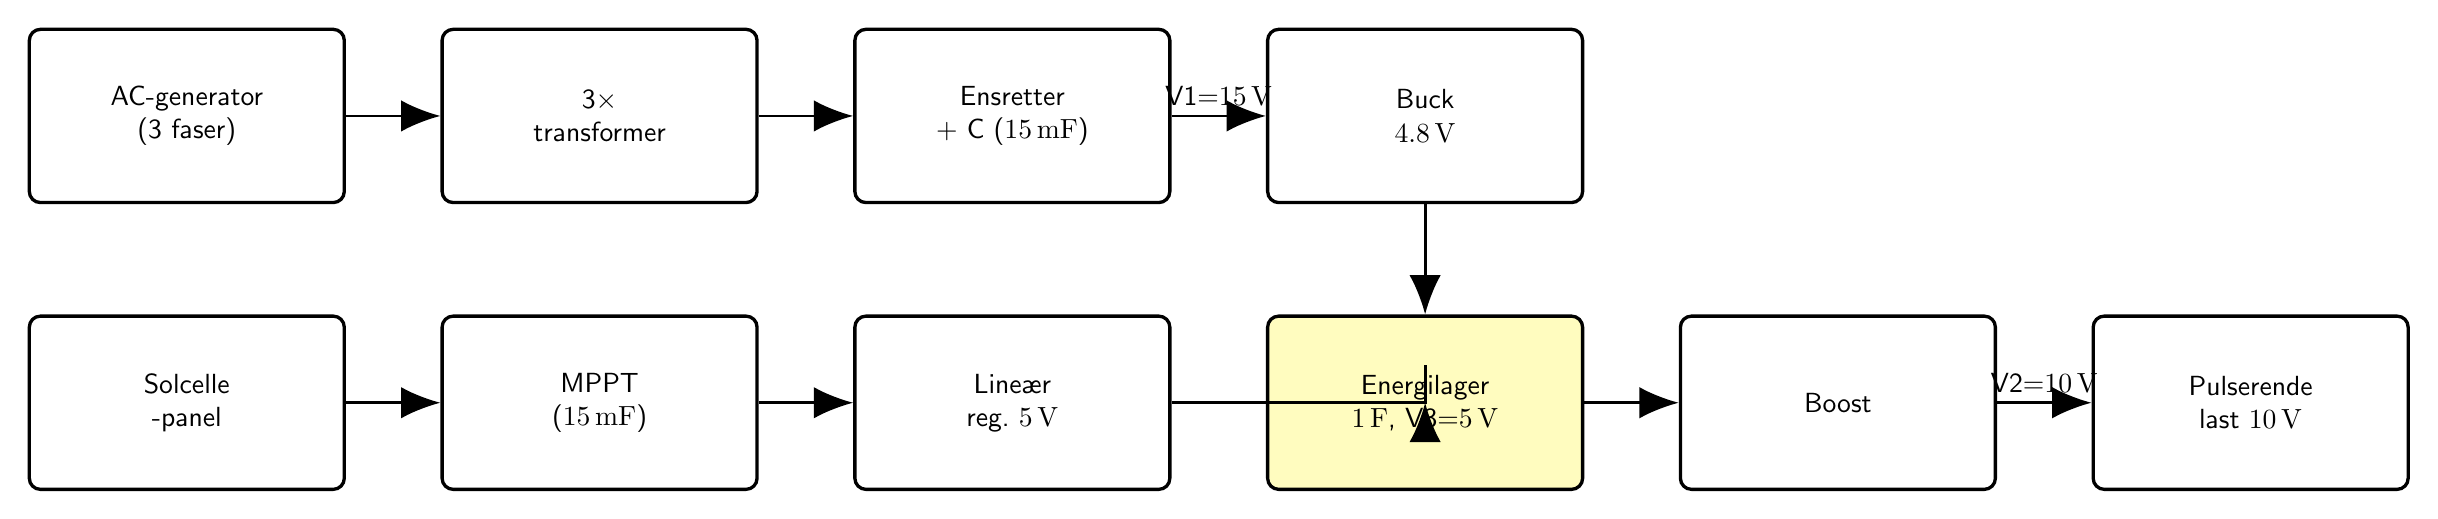
\begin{tikzpicture}[
      node distance = 8mm and 12mm,
      blk/.style = {draw, very thick, rounded corners, align=center,
                    minimum height=22mm, minimum width=40mm, fill=white},
      sto/.style = {blk, fill=yellow!25},
      >={Latex[length=5mm,width=4mm]}, line width=1pt
    ]
    % øvre kæde: generator
    \node[blk] (gen)  {AC-generator\\(3 faser)};
    \node[blk, right=of gen] (tr)   {3$\times$\\transformer};
    \node[blk, right=of tr]  (rec)  {Ensretter\\+ C (\SI{15}{mF})};
    \node[blk, right=of rec] (buck) {Buck\\\SI{4.8}{V}};
    % lager + udgang
    \node[sto, below=14mm of buck] (sto)  {Energilager\\\SI{1}{F}, V3=\SI{5}{V}};
    \node[blk, right=of sto] (boost) {Boost};
    \node[blk, right=of boost] (load) {Pulserende\\last \SI{10}{V}};
    % nedre kæde: solceller
    \node[blk, below=14mm of gen] (sol)  {Solcelle\\-panel};
    \node[blk, right=of sol] (mppt) {MPPT\\(\SI{15}{mF})};
    \node[blk, right=of mppt] (lin) {Lineær\\reg.\ \SI{5}{V}};
    % forbindelser
    \draw[->] (gen)  -- (tr);
    \draw[->] (tr)   -- (rec);
    \draw[->] (rec)  -- node[above]{V1=\SI{15}{V}} (buck);
    \draw[->] (buck) -- (sto);
    \draw[->] (sol)  -- (mppt);
    \draw[->] (mppt) -- (lin);
    \draw[->] (lin)  -| (sto);
    \draw[->] (sto)  -- (boost);
    \draw[->] (boost)-- node[above]{V2=\SI{10}{V}} (load);
  \end{tikzpicture}
  \end{center}\end{fadebox}
  \caption{Blokdiagram af energisystemet: generator- og solcellekæde, fælles
  energilager, og boost-konverter til den pulserende last.}
  \label{fig:blokdiagram}
\end{figure}

\section{Delsystemer}
\begin{itemize}
  \item AC-generator, 3$\times$ transformer og ensretter \,($V_1=\SI{15}{V}$)
  \item Selvbygget buck-konverter (\SI{4.8}{V}) og boost-konverter (\SI{10}{V})
  \item Solcelle + MPPT + lineær regulator \,($V_3=\SI{5}{V}$)
  \item Strømmåling med diskrete komponenter (op-amps tilladt)
  \item Arduino-baseret PID-styring og overvågning
\end{itemize}

\section{Nøglekrav}
\begin{table}
\caption{Centrale spændingskrav (uddrag). Fuld liste i kravspecifikationen.}
\label{tab:krav}
\begin{tabular}{lll}
\toprule
\textbf{Knude} & \textbf{Spænding} & \textbf{Krav} \\
\midrule
$V_1$ & \SI{15}{V} $\pm$\,\SI{1}{V}   & \SIrange{100}{300}{mA}, $<\SI{1.0}{s}$ \\
$V_2$ & \SI{10}{V} $\pm$\,\SI{1}{V}   & $\geq\SI{150}{mA}$, last-step \SIrange{50}{150}{mA} \\
$V_3$ & \SI{5}{V}  $\pm$\,\SI{0.5}{V} & for strømme $>\SI{20}{mA}$ \\
\bottomrule
\end{tabular}
\end{table}

\section{Styring og software}
En Arduino lukker en PID-løkke om motoren via en PWM-driver, så generatoren holdes
på det ønskede arbejdspunkt. Firmwaren bygger på ADC-sampling, timer-interrupts og
PWM-generering. Et PC-baseret system overvåger spændingerne med opdatering hvert
sekund.

\section{Resultater}
\begin{figure}
  \begin{fadebox}\begin{center}
    \vspace{6cm}
    \textbf{[ Måleresultater / plots indsættes her ]}
    \vspace{6cm}
  \end{center}\end{fadebox}
  \caption{Måleresultater for V1/V2/V3 under belastning samt last-respons
  (indsæt grafer fra \texttt{measurements/}).}
  \label{fig:resultater}
\end{figure}

\section{Test og konklusion}
Systemet testes samlet ved at drive et \SI{100}{W} LED-lys (\SI{0.5}{m}) fra
solcellepanelet. \emph{[Opsummér kravopfyldelse: V1/V2/V3 inden for tolerance,
last-respons inden for \SI{1.0}{s}, korrekt energikilde-prioritering (solcelle
først), og samlet virkningsgrad.]}

\end{dtupostercontent}
\end{document}
